% Created by tikzDevice version 0.12.3.1 on 2022-04-16 18:17:23
% !TEX encoding = UTF-8 Unicode
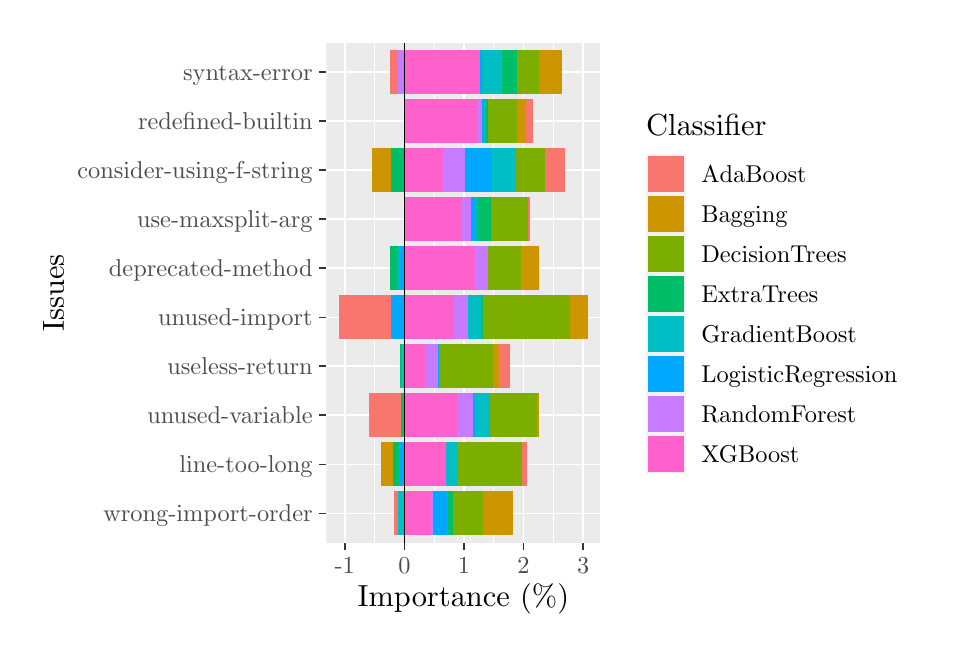
\begin{tikzpicture}[x=1pt,y=1pt]
\definecolor{fillColor}{RGB}{255,255,255}
\path[use as bounding box,fill=fillColor,fill opacity=0.00] (0,0) rectangle (325.21,216.81);
\begin{scope}
\path[clip] (  0.00,  0.00) rectangle (325.21,216.81);
\definecolor{drawColor}{RGB}{255,255,255}
\definecolor{fillColor}{RGB}{255,255,255}

\path[draw=drawColor,line width= 0.6pt,line join=round,line cap=round,fill=fillColor] (  0.00,  0.00) rectangle (325.21,216.81);
\end{scope}
\begin{scope}
\path[clip] (107.91, 30.69) rectangle (206.96,211.31);
\definecolor{fillColor}{gray}{0.92}

\path[fill=fillColor] (107.91, 30.69) rectangle (206.96,211.31);
\definecolor{drawColor}{RGB}{255,255,255}

\path[draw=drawColor,line width= 0.3pt,line join=round] (125.34, 30.69) --
	(125.34,211.31);

\path[draw=drawColor,line width= 0.3pt,line join=round] (146.88, 30.69) --
	(146.88,211.31);

\path[draw=drawColor,line width= 0.3pt,line join=round] (168.42, 30.69) --
	(168.42,211.31);

\path[draw=drawColor,line width= 0.3pt,line join=round] (189.97, 30.69) --
	(189.97,211.31);

\path[draw=drawColor,line width= 0.6pt,line join=round] (107.91, 41.31) --
	(206.96, 41.31);

\path[draw=drawColor,line width= 0.6pt,line join=round] (107.91, 59.02) --
	(206.96, 59.02);

\path[draw=drawColor,line width= 0.6pt,line join=round] (107.91, 76.73) --
	(206.96, 76.73);

\path[draw=drawColor,line width= 0.6pt,line join=round] (107.91, 94.44) --
	(206.96, 94.44);

\path[draw=drawColor,line width= 0.6pt,line join=round] (107.91,112.14) --
	(206.96,112.14);

\path[draw=drawColor,line width= 0.6pt,line join=round] (107.91,129.85) --
	(206.96,129.85);

\path[draw=drawColor,line width= 0.6pt,line join=round] (107.91,147.56) --
	(206.96,147.56);

\path[draw=drawColor,line width= 0.6pt,line join=round] (107.91,165.27) --
	(206.96,165.27);

\path[draw=drawColor,line width= 0.6pt,line join=round] (107.91,182.98) --
	(206.96,182.98);

\path[draw=drawColor,line width= 0.6pt,line join=round] (107.91,200.69) --
	(206.96,200.69);

\path[draw=drawColor,line width= 0.6pt,line join=round] (114.57, 30.69) --
	(114.57,211.31);

\path[draw=drawColor,line width= 0.6pt,line join=round] (136.11, 30.69) --
	(136.11,211.31);

\path[draw=drawColor,line width= 0.6pt,line join=round] (157.65, 30.69) --
	(157.65,211.31);

\path[draw=drawColor,line width= 0.6pt,line join=round] (179.19, 30.69) --
	(179.19,211.31);

\path[draw=drawColor,line width= 0.6pt,line join=round] (200.74, 30.69) --
	(200.74,211.31);
\definecolor{fillColor}{RGB}{248,118,109}

\path[fill=fillColor] (130.94,192.72) rectangle (133.53,208.65);

\path[fill=fillColor] (180.06,175.01) rectangle (182.64,190.95);

\path[fill=fillColor] (186.95,157.30) rectangle (194.27,173.24);

\path[fill=fillColor] (180.70,139.59) rectangle (181.35,155.53);

\path[fill=fillColor] (184.80,121.88) rectangle (184.80,137.82);

\path[fill=fillColor] (112.41,104.18) rectangle (131.37,120.11);

\path[fill=fillColor] (170.15, 86.47) rectangle (174.24,102.40);

\path[fill=fillColor] (123.40, 68.76) rectangle (135.03, 84.70);

\path[fill=fillColor] (178.76, 51.05) rectangle (180.27, 66.99);

\path[fill=fillColor] (132.45, 33.34) rectangle (133.96, 49.28);
\definecolor{fillColor}{RGB}{205,150,0}

\path[fill=fillColor] (184.80,192.72) rectangle (192.98,208.65);

\path[fill=fillColor] (176.82,175.01) rectangle (180.06,190.95);

\path[fill=fillColor] (124.26,157.30) rectangle (131.16,173.24);

\path[fill=fillColor] (180.70,139.59) rectangle (180.70,155.53);

\path[fill=fillColor] (178.12,121.88) rectangle (184.80,137.82);

\path[fill=fillColor] (196.00,104.18) rectangle (202.46,120.11);

\path[fill=fillColor] (168.21, 86.47) rectangle (170.15,102.40);

\path[fill=fillColor] (184.15, 68.76) rectangle (184.80, 84.70);

\path[fill=fillColor] (127.71, 51.05) rectangle (132.02, 66.99);

\path[fill=fillColor] (164.55, 33.34) rectangle (175.32, 49.28);
\definecolor{fillColor}{RGB}{124,174,0}

\path[fill=fillColor] (176.82,192.72) rectangle (184.80,208.65);

\path[fill=fillColor] (166.48,175.01) rectangle (176.82,190.95);

\path[fill=fillColor] (175.96,157.30) rectangle (186.95,173.24);

\path[fill=fillColor] (167.35,139.59) rectangle (180.70,155.53);

\path[fill=fillColor] (166.27,121.88) rectangle (178.12,137.82);

\path[fill=fillColor] (164.55,104.18) rectangle (196.00,120.11);

\path[fill=fillColor] (148.39, 86.47) rectangle (168.21,102.40);

\path[fill=fillColor] (166.92, 68.76) rectangle (184.15, 84.70);

\path[fill=fillColor] (155.28, 51.05) rectangle (178.76, 66.99);

\path[fill=fillColor] (153.77, 33.34) rectangle (164.55, 49.28);
\definecolor{fillColor}{RGB}{0,190,103}

\path[fill=fillColor] (171.44,192.72) rectangle (176.82,208.65);

\path[fill=fillColor] (165.41,175.01) rectangle (166.48,190.95);

\path[fill=fillColor] (131.16,157.30) rectangle (136.11,173.24);

\path[fill=fillColor] (162.39,139.59) rectangle (167.35,155.53);

\path[fill=fillColor] (130.94,121.88) rectangle (133.96,137.82);

\path[fill=fillColor] (163.90,104.18) rectangle (164.55,120.11);

\path[fill=fillColor] (134.39, 86.47) rectangle (135.03,102.40);

\path[fill=fillColor] (135.03, 68.76) rectangle (136.11, 84.70);

\path[fill=fillColor] (132.02, 51.05) rectangle (134.17, 66.99);

\path[fill=fillColor] (151.84, 33.34) rectangle (153.77, 49.28);
\definecolor{fillColor}{RGB}{0,191,196}

\path[fill=fillColor] (164.33,192.72) rectangle (171.44,208.65);

\path[fill=fillColor] (164.76,175.01) rectangle (165.41,190.95);

\path[fill=fillColor] (167.78,157.30) rectangle (175.96,173.24);

\path[fill=fillColor] (162.18,139.59) rectangle (162.39,155.53);

\path[fill=fillColor] (133.96,121.88) rectangle (134.17,137.82);

\path[fill=fillColor] (158.95,104.18) rectangle (163.90,120.11);

\path[fill=fillColor] (135.03, 86.47) rectangle (136.11,102.40);

\path[fill=fillColor] (161.75, 68.76) rectangle (166.92, 84.70);

\path[fill=fillColor] (151.19, 51.05) rectangle (155.28, 66.99);

\path[fill=fillColor] (133.96, 33.34) rectangle (136.11, 49.28);
\definecolor{fillColor}{RGB}{0,169,255}

\path[fill=fillColor] (163.47,192.72) rectangle (164.33,208.65);

\path[fill=fillColor] (164.12,175.01) rectangle (164.76,190.95);

\path[fill=fillColor] (158.08,157.30) rectangle (167.78,173.24);

\path[fill=fillColor] (160.24,139.59) rectangle (162.18,155.53);

\path[fill=fillColor] (134.17,121.88) rectangle (136.11,137.82);

\path[fill=fillColor] (131.37,104.18) rectangle (136.11,120.11);

\path[fill=fillColor] (148.17, 86.47) rectangle (148.39,102.40);

\path[fill=fillColor] (160.88, 68.76) rectangle (161.75, 84.70);

\path[fill=fillColor] (134.17, 51.05) rectangle (136.11, 66.99);

\path[fill=fillColor] (146.45, 33.34) rectangle (151.84, 49.28);
\definecolor{fillColor}{RGB}{199,124,255}

\path[fill=fillColor] (133.53,192.72) rectangle (136.11,208.65);

\path[fill=fillColor] (162.39,175.01) rectangle (164.12,190.95);

\path[fill=fillColor] (150.11,157.30) rectangle (158.08,173.24);

\path[fill=fillColor] (156.79,139.59) rectangle (160.24,155.53);

\path[fill=fillColor] (161.75,121.88) rectangle (166.27,137.82);

\path[fill=fillColor] (154.21,104.18) rectangle (158.95,120.11);

\path[fill=fillColor] (143.43, 86.47) rectangle (148.17,102.40);

\path[fill=fillColor] (155.28, 68.76) rectangle (160.88, 84.70);

\path[fill=fillColor] (151.19, 51.05) rectangle (151.19, 66.99);

\path[fill=fillColor] (145.80, 33.34) rectangle (146.45, 49.28);
\definecolor{fillColor}{RGB}{255,97,204}

\path[fill=fillColor] (136.11,192.72) rectangle (163.47,208.65);

\path[fill=fillColor] (136.11,175.01) rectangle (162.39,190.95);

\path[fill=fillColor] (136.11,157.30) rectangle (150.11,173.24);

\path[fill=fillColor] (136.11,139.59) rectangle (156.79,155.53);

\path[fill=fillColor] (136.11,121.88) rectangle (161.75,137.82);

\path[fill=fillColor] (136.11,104.18) rectangle (154.21,120.11);

\path[fill=fillColor] (136.11, 86.47) rectangle (143.43,102.40);

\path[fill=fillColor] (136.11, 68.76) rectangle (155.28, 84.70);

\path[fill=fillColor] (136.11, 51.05) rectangle (151.19, 66.99);

\path[fill=fillColor] (136.11, 33.34) rectangle (145.80, 49.28);
\definecolor{drawColor}{RGB}{0,0,0}

\path[draw=drawColor,line width= 0.6pt,line join=round] (136.11, 30.69) -- (136.11,211.31);
\end{scope}
\begin{scope}
\path[clip] (  0.00,  0.00) rectangle (325.21,216.81);
\definecolor{drawColor}{gray}{0.30}

\node[text=drawColor,anchor=base east,inner sep=0pt, outer sep=0pt, scale=  0.88] at (102.96, 38.28) {wrong-import-order};

\node[text=drawColor,anchor=base east,inner sep=0pt, outer sep=0pt, scale=  0.88] at (102.96, 55.99) {line-too-long};

\node[text=drawColor,anchor=base east,inner sep=0pt, outer sep=0pt, scale=  0.88] at (102.96, 73.70) {unused-variable};

\node[text=drawColor,anchor=base east,inner sep=0pt, outer sep=0pt, scale=  0.88] at (102.96, 91.41) {useless-return};

\node[text=drawColor,anchor=base east,inner sep=0pt, outer sep=0pt, scale=  0.88] at (102.96,109.11) {unused-import};

\node[text=drawColor,anchor=base east,inner sep=0pt, outer sep=0pt, scale=  0.88] at (102.96,126.82) {deprecated-method};

\node[text=drawColor,anchor=base east,inner sep=0pt, outer sep=0pt, scale=  0.88] at (102.96,144.53) {use-maxsplit-arg};

\node[text=drawColor,anchor=base east,inner sep=0pt, outer sep=0pt, scale=  0.88] at (102.96,162.24) {consider-using-f-string};

\node[text=drawColor,anchor=base east,inner sep=0pt, outer sep=0pt, scale=  0.88] at (102.96,179.95) {redefined-builtin};

\node[text=drawColor,anchor=base east,inner sep=0pt, outer sep=0pt, scale=  0.88] at (102.96,197.65) {syntax-error};
\end{scope}
\begin{scope}
\path[clip] (  0.00,  0.00) rectangle (325.21,216.81);
\definecolor{drawColor}{gray}{0.20}

\path[draw=drawColor,line width= 0.6pt,line join=round] (105.16, 41.31) --
	(107.91, 41.31);

\path[draw=drawColor,line width= 0.6pt,line join=round] (105.16, 59.02) --
	(107.91, 59.02);

\path[draw=drawColor,line width= 0.6pt,line join=round] (105.16, 76.73) --
	(107.91, 76.73);

\path[draw=drawColor,line width= 0.6pt,line join=round] (105.16, 94.44) --
	(107.91, 94.44);

\path[draw=drawColor,line width= 0.6pt,line join=round] (105.16,112.14) --
	(107.91,112.14);

\path[draw=drawColor,line width= 0.6pt,line join=round] (105.16,129.85) --
	(107.91,129.85);

\path[draw=drawColor,line width= 0.6pt,line join=round] (105.16,147.56) --
	(107.91,147.56);

\path[draw=drawColor,line width= 0.6pt,line join=round] (105.16,165.27) --
	(107.91,165.27);

\path[draw=drawColor,line width= 0.6pt,line join=round] (105.16,182.98) --
	(107.91,182.98);

\path[draw=drawColor,line width= 0.6pt,line join=round] (105.16,200.69) --
	(107.91,200.69);
\end{scope}
\begin{scope}
\path[clip] (  0.00,  0.00) rectangle (325.21,216.81);
\definecolor{drawColor}{gray}{0.20}

\path[draw=drawColor,line width= 0.6pt,line join=round] (114.57, 27.94) --
	(114.57, 30.69);

\path[draw=drawColor,line width= 0.6pt,line join=round] (136.11, 27.94) --
	(136.11, 30.69);

\path[draw=drawColor,line width= 0.6pt,line join=round] (157.65, 27.94) --
	(157.65, 30.69);

\path[draw=drawColor,line width= 0.6pt,line join=round] (179.19, 27.94) --
	(179.19, 30.69);

\path[draw=drawColor,line width= 0.6pt,line join=round] (200.74, 27.94) --
	(200.74, 30.69);
\end{scope}
\begin{scope}
\path[clip] (  0.00,  0.00) rectangle (325.21,216.81);
\definecolor{drawColor}{gray}{0.30}

\node[text=drawColor,anchor=base,inner sep=0pt, outer sep=0pt, scale=  0.88] at (114.57, 19.68) {-1};

\node[text=drawColor,anchor=base,inner sep=0pt, outer sep=0pt, scale=  0.88] at (136.11, 19.68) {0};

\node[text=drawColor,anchor=base,inner sep=0pt, outer sep=0pt, scale=  0.88] at (157.65, 19.68) {1};

\node[text=drawColor,anchor=base,inner sep=0pt, outer sep=0pt, scale=  0.88] at (179.19, 19.68) {2};

\node[text=drawColor,anchor=base,inner sep=0pt, outer sep=0pt, scale=  0.88] at (200.74, 19.68) {3};
\end{scope}
\begin{scope}
\path[clip] (  0.00,  0.00) rectangle (325.21,216.81);
\definecolor{drawColor}{RGB}{0,0,0}

\node[text=drawColor,anchor=base,inner sep=0pt, outer sep=0pt, scale=  1.10] at (157.44,  7.64) {Importance (\%)};
\end{scope}
\begin{scope}
\path[clip] (  0.00,  0.00) rectangle (325.21,216.81);
\definecolor{drawColor}{RGB}{0,0,0}

\node[text=drawColor,rotate= 90.00,anchor=base,inner sep=0pt, outer sep=0pt, scale=  1.10] at ( 13.08,121.00) {Issues};
\end{scope}
\begin{scope}
\path[clip] (  0.00,  0.00) rectangle (325.21,216.81);
\definecolor{fillColor}{RGB}{255,255,255}

\path[fill=fillColor] (217.96, 50.07) rectangle (319.71,191.92);
\end{scope}
\begin{scope}
\path[clip] (  0.00,  0.00) rectangle (325.21,216.81);
\definecolor{drawColor}{RGB}{0,0,0}

\node[text=drawColor,anchor=base west,inner sep=0pt, outer sep=0pt, scale=  1.10] at (223.46,177.78) {Classifier};
\end{scope}
\begin{scope}
\path[clip] (  0.00,  0.00) rectangle (325.21,216.81);
\definecolor{fillColor}{gray}{0.95}

\path[fill=fillColor] (223.46,156.75) rectangle (237.92,171.21);
\end{scope}
\begin{scope}
\path[clip] (  0.00,  0.00) rectangle (325.21,216.81);
\definecolor{fillColor}{RGB}{248,118,109}

\path[fill=fillColor] (224.17,157.46) rectangle (237.21,170.50);
\end{scope}
\begin{scope}
\path[clip] (  0.00,  0.00) rectangle (325.21,216.81);
\definecolor{fillColor}{gray}{0.95}

\path[fill=fillColor] (223.46,142.30) rectangle (237.92,156.75);
\end{scope}
\begin{scope}
\path[clip] (  0.00,  0.00) rectangle (325.21,216.81);
\definecolor{fillColor}{RGB}{205,150,0}

\path[fill=fillColor] (224.17,143.01) rectangle (237.21,156.04);
\end{scope}
\begin{scope}
\path[clip] (  0.00,  0.00) rectangle (325.21,216.81);
\definecolor{fillColor}{gray}{0.95}

\path[fill=fillColor] (223.46,127.84) rectangle (237.92,142.30);
\end{scope}
\begin{scope}
\path[clip] (  0.00,  0.00) rectangle (325.21,216.81);
\definecolor{fillColor}{RGB}{124,174,0}

\path[fill=fillColor] (224.17,128.56) rectangle (237.21,141.59);
\end{scope}
\begin{scope}
\path[clip] (  0.00,  0.00) rectangle (325.21,216.81);
\definecolor{fillColor}{gray}{0.95}

\path[fill=fillColor] (223.46,113.39) rectangle (237.92,127.84);
\end{scope}
\begin{scope}
\path[clip] (  0.00,  0.00) rectangle (325.21,216.81);
\definecolor{fillColor}{RGB}{0,190,103}

\path[fill=fillColor] (224.17,114.10) rectangle (237.21,127.13);
\end{scope}
\begin{scope}
\path[clip] (  0.00,  0.00) rectangle (325.21,216.81);
\definecolor{fillColor}{gray}{0.95}

\path[fill=fillColor] (223.46, 98.94) rectangle (237.92,113.39);
\end{scope}
\begin{scope}
\path[clip] (  0.00,  0.00) rectangle (325.21,216.81);
\definecolor{fillColor}{RGB}{0,191,196}

\path[fill=fillColor] (224.17, 99.65) rectangle (237.21,112.68);
\end{scope}
\begin{scope}
\path[clip] (  0.00,  0.00) rectangle (325.21,216.81);
\definecolor{fillColor}{gray}{0.95}

\path[fill=fillColor] (223.46, 84.48) rectangle (237.92, 98.94);
\end{scope}
\begin{scope}
\path[clip] (  0.00,  0.00) rectangle (325.21,216.81);
\definecolor{fillColor}{RGB}{0,169,255}

\path[fill=fillColor] (224.17, 85.19) rectangle (237.21, 98.23);
\end{scope}
\begin{scope}
\path[clip] (  0.00,  0.00) rectangle (325.21,216.81);
\definecolor{fillColor}{gray}{0.95}

\path[fill=fillColor] (223.46, 70.03) rectangle (237.92, 84.48);
\end{scope}
\begin{scope}
\path[clip] (  0.00,  0.00) rectangle (325.21,216.81);
\definecolor{fillColor}{RGB}{199,124,255}

\path[fill=fillColor] (224.17, 70.74) rectangle (237.21, 83.77);
\end{scope}
\begin{scope}
\path[clip] (  0.00,  0.00) rectangle (325.21,216.81);
\definecolor{fillColor}{gray}{0.95}

\path[fill=fillColor] (223.46, 55.57) rectangle (237.92, 70.03);
\end{scope}
\begin{scope}
\path[clip] (  0.00,  0.00) rectangle (325.21,216.81);
\definecolor{fillColor}{RGB}{255,97,204}

\path[fill=fillColor] (224.17, 56.29) rectangle (237.21, 69.32);
\end{scope}
\begin{scope}
\path[clip] (  0.00,  0.00) rectangle (325.21,216.81);
\definecolor{drawColor}{RGB}{0,0,0}

\node[text=drawColor,anchor=base west,inner sep=0pt, outer sep=0pt, scale=  0.88] at (243.42,160.95) {AdaBoost};
\end{scope}
\begin{scope}
\path[clip] (  0.00,  0.00) rectangle (325.21,216.81);
\definecolor{drawColor}{RGB}{0,0,0}

\node[text=drawColor,anchor=base west,inner sep=0pt, outer sep=0pt, scale=  0.88] at (243.42,146.50) {Bagging};
\end{scope}
\begin{scope}
\path[clip] (  0.00,  0.00) rectangle (325.21,216.81);
\definecolor{drawColor}{RGB}{0,0,0}

\node[text=drawColor,anchor=base west,inner sep=0pt, outer sep=0pt, scale=  0.88] at (243.42,132.04) {DecisionTrees};
\end{scope}
\begin{scope}
\path[clip] (  0.00,  0.00) rectangle (325.21,216.81);
\definecolor{drawColor}{RGB}{0,0,0}

\node[text=drawColor,anchor=base west,inner sep=0pt, outer sep=0pt, scale=  0.88] at (243.42,117.59) {ExtraTrees};
\end{scope}
\begin{scope}
\path[clip] (  0.00,  0.00) rectangle (325.21,216.81);
\definecolor{drawColor}{RGB}{0,0,0}

\node[text=drawColor,anchor=base west,inner sep=0pt, outer sep=0pt, scale=  0.88] at (243.42,103.13) {GradientBoost};
\end{scope}
\begin{scope}
\path[clip] (  0.00,  0.00) rectangle (325.21,216.81);
\definecolor{drawColor}{RGB}{0,0,0}

\node[text=drawColor,anchor=base west,inner sep=0pt, outer sep=0pt, scale=  0.88] at (243.42, 88.68) {LogisticRegression};
\end{scope}
\begin{scope}
\path[clip] (  0.00,  0.00) rectangle (325.21,216.81);
\definecolor{drawColor}{RGB}{0,0,0}

\node[text=drawColor,anchor=base west,inner sep=0pt, outer sep=0pt, scale=  0.88] at (243.42, 74.23) {RandomForest};
\end{scope}
\begin{scope}
\path[clip] (  0.00,  0.00) rectangle (325.21,216.81);
\definecolor{drawColor}{RGB}{0,0,0}

\node[text=drawColor,anchor=base west,inner sep=0pt, outer sep=0pt, scale=  0.88] at (243.42, 59.77) {XGBoost};
\end{scope}
\end{tikzpicture}
